% tirlnx01 - Materiaal om het keuzevak Linux te geven 
% op de Hogeschool Rotterdam.
% Copyright (C) 2010 - 2011  Paul Sohier, Kevin van der Vlist
%
% This program is free software: you can redistribute it and/or modify
% it under the terms of the GNU General Public License as published by
% the Free Software Foundation, either version 3 of the License, or
% (at your option) any later version.
%
% This program is distributed in the hope that it will be useful,
% but WITHOUT ANY WARRANTY; without even the implied warranty of
% MERCHANTABILITY or FITNESS FOR A PARTICULAR PURPOSE.  See the
% GNU General Public License for more details.
%
% You should have received a copy of the GNU General Public License
% along with this program.  If not, see <http://www.gnu.org/licenses/>.
%
% Kevin van der Vlist - kevin@kevinvandervlist.nl
% Paul Sohier - paul@paulsohier.nl

\chapter{Shell}
\section{Inleiding shell}
\begin{figure}[H]
  \begin{center}
    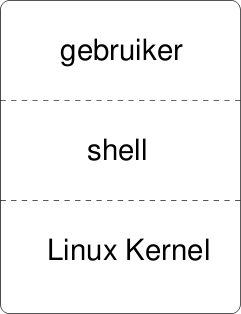
\includegraphics[scale=0.5]{images/shell_intro}
  \end{center}
  \caption{De basis}
  \label{fig:shell}
\end{figure}

De \emph{shell} staat tussen de gebruiker en het systeem in en dient als \emph{opdrachtinterpreter}. De \emph{shell} hiermee vergelijkbaar met \emph{command.com} onder \emph{DOS}. Wanneer een gebruiker een commando geeft controleerd de \emph{shell} of dit opgegeven commando correct is. Hierna zal de \emph{shell} de opdracht uitvoeren, of een foutmelding teruggeven naar de gebruiker. De \emph{shell} is hiermee de eerste laag in het besturings systeem. 

Op elk systeem is er een \emph{shell} die ervoor zorgt dat commando's worden uitgevoerd. Onder \emph{Linux} zijn er meerdere \emph{shells} zoals bijvoorbeeld de \emph{Bash-Shell}, \emph{Korn-shell} en de \emph{C-shell}.

De \emph{Bourne shell} is de \emph{shell} die origineel op de \emph{AT\&T UNIX} systemen stond onder de naam sh. \emph{Bourne Again Shell} (\texttt{bash}\index{bash}) is de opensource versie en is compitable met het orgineel. Deze \emph{shell} heeft echter wel extra mogelijkheden\footnote{Bourne Again SHell, de hoofdletters ``hell'' slaan op de problemen die sommige ermee hebben}.

Naast \emph{Bash} zijn er tegenwoordig ook nog andere afgeleiden. Een goed voorbeeld hiervan is \texttt{dash}\index{dash}, \emph{Debian Almquist Shell}. Dash komt af van de in \emph{netBSD} bekende \emph{Almquist Shell} en was naar \emph{Linux} geport in 2002 \cite{bib.dash}. Het voordeel van Dash is dat het een stuk sneller is als \emph{Bash}, maar toch nog werkt volgens de \emph{POSIX} standard.\index{POSIX} Tegenwoordig maken bijvoorbeeld \emph{Debian}\footnote{\emph{Debian} maakt vanaf de \emph{Debian Squeeze} release standaard gebruik van \emph{Dash}.} en \emph{Ubuntu} gebruik van Dash.

Een \emph{Linux} systeem is geen systeem zonder een \emph{shell}, en de scripting mogelijkheden die daardoor aanwezig zijn. Bijna alles is opgebouwd rond de \emph{shell}. Een goed voorbeeld hiervan zijn de opstart scripts in \emph{Slackware}\footnote{Dit geldt natuurlijk ook voor andere distributies}. Hieronder is een voorbeeld \emph{init} script van de \emph{OpenSSH Server}:
\begin{lstlisting}
root@slackje:/etc/rc.d# cat rc.sshd 
#!/bin/sh
# Start/stop/restart the secure shell server:

sshd_start() {
  # Create host keys if needed.
  if [ ! -r /etc/ssh/ssh_host_key ]; then
    /usr/bin/ssh-keygen -t rsa1 -f /etc/ssh/ssh_host_key -N '' 
  fi
  if [ ! -f /etc/ssh/ssh_host_dsa_key ]; then
    /usr/bin/ssh-keygen -t dsa -f /etc/ssh/ssh_host_dsa_key -N ''
  fi
  if [ ! -f /etc/ssh/ssh_host_rsa_key ]; then
    /usr/bin/ssh-keygen -t rsa -f /etc/ssh/ssh_host_rsa_key -N ''
  fi
  /usr/sbin/sshd
}

sshd_stop() {
  killall sshd
}

sshd_restart() {
  if [ -r /var/run/sshd.pid ]; then
    echo "WARNING: killing listener process only.  To kill every sshd process, you must"
    echo "         use 'rc.sshd stop'.  'rc.sshd restart' kills only the parent sshd to"
    echo "         allow an admin logged in through sshd to use 'rc.sshd restart' without"
    echo "         being cut off.  If sshd has been upgraded, new connections will now"
    echo "         use the new version, which should be a safe enough approach."
    kill `cat /var/run/sshd.pid`
  else
    echo "WARNING: There does not appear to be a parent instance of sshd running."
    echo "         If you really want to kill all running instances of sshd (including"
    echo "         any sessions currently in use), run '/etc/rc.d/rc.sshd stop' instead."
    exit 1
  fi
  sleep 1
  sshd_start
}

case "$1" in
'start')
  sshd_start
  ;;
'stop')
  sshd_stop
  ;;
'restart')
  sshd_restart
  ;;
*)
  echo "usage $0 start|stop|restart"
esac
\end{lstlisting}
Het bovenstaande script zal waarschijnlijk niet helemaal direct begrijpbaar zijn. Wel zullen de grote lijnen al zichtbaar zijn. In de volgende twee hoofdstukken zal de \emph{shell} behandeld worden, waarna het bovenstaande script duidelijk te begrijpen is. Ook zal het maken van eigen scripts hierna mogelijk zijn. 

\emph{Shell} scripting is een van de sterkste punten van \emph{Linux}, omdat het gebruikers en beheerders in staat stelt een systeem ontzettend flexibel te houden. Ook kan het laagdrempelig aan worden gepast naar eigen, specifieke wensen. 

\section{De theorie}
Voordat er uitgebreid begonnen wordt met het bespreken van de verschillende mogelijkheden in de \emph{shell} is het belangerijk om te begrijpen hoe de \emph{shell} precies werkt en wat de eisen zijn. Een uitstekende documentatie over de \emph{shell} is te vinden via \texttt{man}\index{man} \texttt{bash}\index{bash}. Hierin is een goede uitleg te vinden over de werking van de \emph{shell}. Het is mogelijk om uitgebreidere documentatie gerelateerd aan scripting op te zoeken. Een goede plek hiervoor is \emph{tldp}\cite{bib.tldp.abs}, een compleet overzicht van de functionaliteit van de \emph{Bash shell}. 

De meeste generieke beschrijving van een \emph{shell} is als volgt:
\begin{quote}
any program that users employ to type commands
\end{quote}
In \emph{UNIX} zijn er verschillende soorten \emph{Shells}. Wanneer een gebruiker inlogt in het systeem zal de \emph{shell} automatisch worden gestart. De meeste \emph{Shells} zijn hiervoor special ontwikkeld. Dit programma heet een \emph{Shell} omdat het het onderliggende operating system verbergt achter de interface van de \emph{Shell}. De \emph{Shell} beheerd de technische details van de kernel interface, welke de binnenste laag is binnen elk operating system.

Ook de grafische interfaces, zoals \emph{Gnome}, \emph{KDE} of \emph{Fluxbox} zijn \emph{Shells}. Ze worden ook wel \emph{visuele} \emph{shells} of grafische \emph{shells} genoemd. \cite{bib.shell}

\subsection{Interactive command line en scripting program language?}
Toen de \emph{UNIX shell} voor het eerst uitkwam was dit een bijzondere \emph{shell}. Er waren al wel andere \emph{Shells}, maar de \emph{Shells} welke er al wel waren waren niet en een \emph{Interactive Commandline} en een \emph{Scripting Program Language}. De \emph{UNIX shell} was dit wel, met alle voordelen van dien. Je kon nu zelf programma's draaien met de \emph{Shell} en je had dus een stuk meer vrijheid om dingen te doen. 
 
\subsection{Shebang}
Wanneer een programma gestart wordt moet de file loader van de \emph{Shell} weten waarmee het programma geopend moet worden. Standaard zal dit meestal het programma met de \emph{Shell} waarin op dat moment een gebruiker actief is. 

Het kan voorkomen dat het script met een andere \emph{shell} of binary gestart zal moeten worden. Een andere mogelijkheid is het verkrijgen van een garantie dat een bepaalde \emph{shell} het script start. Om dit doel te bereiken kan er gebruik gemaakt worden van een \emph{shebang}, een speciale eerste regel in een script. Deze \emph{shebang} ziet er als volgt uit:
\begin{lstlisting}
#!/bin/bash
\end{lstlisting}
Het hekje met het uitroepteken is de \emph{shebang}. Doordat het hekje commentaar is, zal het genegeerd worden door de interpreter. De program loader zal het echter wel lezen en de goede interpreter aanroepen. In het geval van hierboven dus de \emph{Bash shell}. Er kan op deze manier bijvoorbeeld ook eenvoudig een \emph{Perl}, \emph{PHP} of andere interpreter aangeroepen worden in de \emph{shell}. 

\subsection{Dash in Slackware?}
De standaard \emph{Shell} in \emph{Slackware} is \emph{Bash}. Het is echter mogelijk een andere \emph{shell} te kiezen. Van de \emph{Dash shell} zijn er in \emph{Slackware} geen standaard paketten, maar Ash\footnote{Dash is afgeleid van Ash} is wel beschikbaar. 

Hieronder is te zien hoe een nieuwe gebruiker wordt aangemaakt, welke gebruik zal maken van de \emph{Ash shell}:
\begin{lstlisting}
root@slackje:~# adduser dashtest
Login name for new user: dashtest
User ID ('UID') [ defaults to next available ]: 
Initial group [ users ]: 
Additional UNIX groups:
[...]
:  
Home directory [ /home/dashtest ] 
Shell [ /bin/bash ] /bin/ash
Expiry date (YYYY-MM-DD) []: 
New account will be created as follows:
---------------------------------------
Login name.......:  dashtest
UID..............:  [ Next available ]
Initial group....:  users
Additional groups:  [ None ]
Home directory...:  /home/dashtest
Shell............:  /bin/ash
Expiry date......:  [ Never ]
\end{lstlisting}
De \emph{Ash shell} uit \emph{Slackware} is niet exact hetzelfde als \emph{Bash} en \emph{Dash}. Na het inloggen zal het eerste verschil al opvallen. Ook zullen dingen als \emph{tab completion} zal niet standaard werken. Andere distributies, zoals \emph{Debian/Ubuntu} zullen standaard instellingen aanbieden waarbij dit wel mogelijk is. Om Ash zich hetzelfde te laten gedragen als \emph{Bash} zal er dus wel het een en ander moeten worden aangepast.

In de rest van dit hoofdstuk wordt er vanuit gegaan dat de standaard \emph{shell} de \emph{Bash shell} is. Het gebruik van een andere \emph{shell} is mogelijk, maar hou rekening met de verschillen tussen de \emph{shells}. 

\subsection{In en output}\index{STDOUT}\index{STDIN}\index{STDERR}
De \emph{shell} heeft, net als ieder ander proces, mogelijkheden tot in-, en output van data. De input, \emph{STDIN}, is bijvoorbeeld het toetsenbord\footnote{Dit kan ook wat anders zijn, zie de paragraaf Piping} of de muis. De output, \emph{STDOUT}, is bijvoorbeeld het scherm, of een bestand. Hiernaast is er ook nog \emph{STDERR}. Op deze \emph{stream} worden de fouten uitgevoerd. De \emph{STDERR} wordt standaard naar het scherm geschreven, maar kan ook worden doorgestuurd naar iets anders als dit nodig is. Deze \emph{streams} kunnen ook in programma's gebruikt worden. In C kunnen deze streams bijvoorbeeld gewoon met \emph{fopen()} benaderd worden. In \ref{fig:output} is een goed voorbeeld te zien van hoe de in/output werkt bij een applicatie. In principe is dit hetzelfde voor alle applicaties.
\begin{figure}[H]
  \begin{center}
    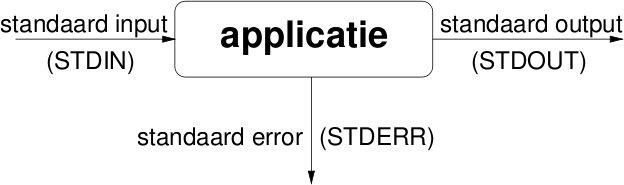
\includegraphics[scale=0.5]{images/inout}
  \end{center}
  \caption{In en Output}
  \label{fig:output}
\end{figure}
Het kunnen gebruiken van deze streams is heel belangrijk voor \emph{Shells}. Zorg dus dat de basis hiervan goed duidelijk is. 

\subsection{Pipeline}
Alle \emph{UNIX} applicaties hebben een standaard input en standaard output mogelijkheid. De \emph{shell} bied handige functionaliteit bij het doorsluizen van uitvoer met het '$|$' teken (sluis, engels: pipe). Het '$|$' teken sluist de uitkomst van de eerste opdracht naar de input van de tweede. Een kort voorbeeld:
\begin{lstlisting}q
  grep kernel /var/log/syslog | more
\end{lstlisting}
\index{cat}\index{grep}\index{more}\index{\textpipe}
\texttt{cat}\index{cat} leest een bestand uit, in dit geval de logfile /var/log/syslog. De output wordt nu gepiped naar het commando \texttt{grep}\index{grep} met een $|$. De output wordt nu niet doorgestuurd naar de \emph{stdout}, en zal dus niet worden weergeven op je scherm. Zodra \texttt{grep}\index{grep} de output ontvangt zoekt \texttt{grep}\index{grep} naar de tekenreeks die opgegeven is. Dat is in dit geval ``kernel''. Voordat het nu doorgestuurd wordt naar de \emph{stdout} wordt het eerst nog gepiped via \texttt{more}\index{more}. \texttt{more}\index{more} zorgt ervoor dat de output gestopt wordt zodra het scherm vol is. Op deze manier kan het resultaat gemakkelijk bekeken worden. Alles gelezen? Dan kan er naar de volgende buffer gegaan worden. 

\begin{lstlisting}
  grep bash /etc/passwd | sort > ~/bash_gebruikers.txt
\end{lstlisting}\index{sort}\index{grep}\index{$>$}
\texttt{grep}\index{grep} ontvangt de inhoud van de file '/etc/passwd' en doorzoekt de inhoud naar de tekenreeks ``bash''. Zit die reeks niet in een regel, dan wordt deze genegeerd. Alle regels van passwd-bestand met ``bash'' in de regels worden nu doorgesluisd naar \texttt{sort}\index{sort}. Deze plaatst ze op alfabetische volgorde. 

Net zoals bij het vorige voorbeeld ontvangt \texttt{grep}\index{grep} weer het resultaat van \texttt{cat}\index{cat}, waarbij het resultaat de inhoud van een bestand is, in dit geval /etc/passwd. Nadat er gezocht is op de string ``bash'' wordt het gepiped naar \texttt{sort}\index{sort}, welke ze sorteert op alfabetische volgorde. 

Het '$>$' teken wordt gebruikt om het resultaat op de \emph{stdout} weg te schrijven. Het resultaat wordt nu naar de file ``bash\_gebruikers'' geschreven. Let wel op dat gebruik maken van '$>$' betekend dat de file, waar de output naartoe wordt gestuurd, gewist zal worden. Om de output achter de huidige content te plakken kan er gebruik gemaakt worden van '$>>$'\index{$>>$}. Wanneer de file niet bestand zal die dan wel gemaakt worden.

Dit soort constructies stellen een gebruiker dus in staat om de uitvoer, \emph{STDOUT} via een \emph{pipeline} als invoer \emph{STDIN} naar het volgende programma te sturen. 

\subsubsection{STDERR redirecten}\index{STDERR}
Hiervoor was al te zien dat \emph{STDOUT} te redirecten is naar een bestand. Maar wat gebeurt er wanneer er fouten optreden? Die moeten misschien ook wel ergens heen. Ook de data op \emph{STDERR} is te redirecten: 
\begin{lstlisting}
cat /etc/passwd | grep test 2> grep_errors.txt
\end{lstlisting}
In het voorbeeld hierboven is te zien dat er geen gebruik gemaakt wordt van $>$ maar van 2$>$\index{2$>$}. Dit houdt in dat de fouten die eventueel optreden worden geschreven naar het bestand ``grep\_errors.txt''. De gewone output wordt nu naar \emph{STDOUT} geschreven. Deze zal niet worden opgeslagen in het bestand.

\begin{lstlisting}
cat /etc/passwd | grep test 1>&2 
\end{lstlisting}
In sommige gevallen is het handig om de output van \emph{STDOUT} te redirecten naar \emph{STDERR}. Dat is precies wat de 1$>$\&2 doet. \index{1$>$\&2}

\begin{lstlisting}
cat /etc/passwd | grep test 2>&1
\end{lstlisting}
Het is vaak veel handiger om dit precies omgekeerd te doen, ofwel de \emph{STDERR} naar \emph{STDOUT} te redirecten. En ook hier is iets voor bedacht, en wel 2$>$\&1 en dus precies het omgekeerde. Let dus goed op de syntax en kies de juiste redirect in de juiste situatie\index{2$>$\&1}.

\begin{lstlisting}
rm tmp/ -rfv &> /dev/null
\end{lstlisting}
\&$>$ zal alle output die vanaf \texttt{rm}\index{rm} afkomt van zowel \emph{STDOUT} als \emph{STDERR} worden redirect naar het opgegeven bestand. In dit geval wordt dit geredirect naar \emph{/dev/null}\index{/dev/null}.

\subsection{TAB-completion}
TAB-completion is eenvoudig en werkt erg makkelijk volgens een simpel principe:
Als er genoeg letters ingevoerd zijn zodat een bestand, opdracht, of naam van een directory kan worden achterhaalt dan vult \emph{Bash} de rest aan. Een voorbeeld:
\begin{lstlisting}
  /usr/lo [tab] wordt /usr/local
\end{lstlisting}
Als er nu op TAB wordt gedrukt vult \emph{Bash} het aan, omdat het ziet dat er gezocht wordt naar '/usr/local'.

Als er bij /usr/li op tab wordt gedrukt kan \emph{Bash} niet het juiste resultaat vinden omdat er meerdere directories zijn die beginnen met /usr/li. Als er vervolgens nogmaals op tab wordt gedrukt geeft \emph{Bash} alle mogelijkheden weer.

\subsection{Opdrachtalliassering}
\begin{lstlisting}
alias psa='ps -aux | less'
alias cp='cp -i'
alias mv='mv -i'
alias rm='rm -i'
\end{lstlisting}
Alias geeft de mogelijkheid om een commando te herschrijven met extra opties. Zet het bovenstaande voorbeeld in het bestand \emph{\~{}/.bash\_profile}\index{\~{}/.bash\_profile} in de home-directory (maak het zonodig aan). Dit bestand zijn extra configuratie instellingen voor de \emph{Bash}B \emph{shell}. Globale \emph{Bash} instellingen moeten in het bestand \emph{/etc/profile} gedaan worden. Activeer de aanpassingen door opnieuw in te loggen of via het commando \texttt{source \~{}/.bash\_profile}.\index{\~{}/.bash\_profile}

\subsection{Historylist}
\emph{Bash} onthoudt bij een sessie de uitgevoerde opdrachten. Bij het uitloggen van het systeem worden alle opdrachten in de file \emph{\~{}/.bash\_history} in de home-directory geschreven. Wanneer een gebruiker de volgende keer inlogt zal door het commando \emph{history}\index{history} precies te zien zijn wat er bij een vorige sessie is gedaan. Als er tijdens een sessie een opdracht uitgevoerd moet worden die al uitgevoerd is kan er met het pijltje-omhoog de vorige opdrachten worden geselecteerd.

Een andere functionaliteit die \emph{Bash} biedt is om een commando dat net is ingegeven te herhalen. Hiervan een korte beschouwing:
\begin{lstlisting}
  mount /dev/hdd -t iso9660 -o ro /mnt/cdrom
\end{lstlisting}
\index{mount}
Omdat dit soort lange opdrachten veel tijd kosten om in te tikken is het gemakkelijk als zo'n opdracht herhaalt moet worden. Door "!$<$commando$>$" te voer je de vorige opdracht uit. In dit geval is dat dus '!mount'.

\subsection{Jobcontrol}
Jobcontrol is mogelijk in \emph{Linux} omdat het een multi-tasking operating system is. Met job control kan in een \emph{shell} meerdere programma's tegelijkertijd worden uitgevoerd. Normaal gesproken draait een opdracht die wordt uitgevoerd op de voorgrond. Met andere worden, de prompt verschijnt pas weer als de opdracht is be\"{e}indigd. De makkelijkstse manier om een job op de achtergrond te plaatsen is door aan het einde van de opdracht een ``\&'' (ampersand) te plaatsen.\index{\&}

De volgende opdracht zoekt vanaf de root ('/') naar alle bestanden die op '.txt' eindigen en zet het resultaat ervan in het bestand 'tekstbestanden'. Doordat er een ampersand achterrstaat wordt het op de achtergrond uitgevoerd en verschijnt de \emph{shell} prompt weer. \texttt{ls -IR /}\index{ls} laat alle bestanden vanaf root zien.\index{ls}

Een op de voorgrond gestart programma kan naar de achtergrond worden gestuurd door \emph{ctrl-z}.
\index{ls}
\begin{lstlisting}
find / -name '*.txt*' > tekstbestanden &
ls -IR / &
\end{lstlisting}
Met de opdracht \index{jobs}\index{jobs} worden alle achtergrond-processen weergeven en in dit geval zou het dus de find opdracht weergeven en de ls opdracht.
\begin{lstlisting}
[1]- Running find / - name '*.txt *' > tekstbestanden &
[2]+ Running ls −lR / &
\end{lstlisting}
Wanneer 'Running' in 'Stopped' veranderd is het process gestopt. Aannemende dat het nog loopt kan het naar de voorgrond gehaald worden met \texttt{fg \%1}\index{fg} of met \texttt{fg find}. Het komt voor dat een lopende opdracht be\"{e}indigd moet worden. Met de opdracht \texttt{kill}\index{kill} is een opdracht af te breken op het \emph{PID} (process ID). Het PID is te zien door \texttt{ps -aux}\index{ps} in te geven. Ook kan \emph{KILL} lopende achtergrond processen stoppen: \index{kill}\texttt{kill \%2} zal in dit geval \texttt{ls -IR /}\index{ls} be\"{e}indigen. Mocht het voorkomen dat alle processen met een bepaalde naam be\"{e}indigd moeten worden dan zou dat het beste met \index{killall}\texttt{killall $<$naam$>$} gedaan kunnen worden.

\subsection{Patronen, Joker-tekens en Accolades}
Een krachtige optie van de \emph{Bash shell} is het gebruik van patronen om bestanden en opdrachten mee aan te duiden.

\begin{lstlisting}
  \* Staat voor 0 of meerdere willekeurige tekens (wildcard, jokerteken)
  \? Staat voor 1 willekeurig teken
  [...] Staat voor 1 van de tekens tussen de haken
  [A-F] Staat voor alle tekens tussen het eerste en tweede
  [!..] Staat voor elk ander teken dan dat er tussen de haken staat
  [!A-F] Staat dus voor elk ander dat niet tussen de A en de F zit
\end{lstlisting}
Alle bestanden van drie letters beginnende met de 'a' en eindigen op de 'z' kunnen gevonden worden met:\index{ls|(}
\begin{lstlisting}
  ls -l a?z
\end{lstlisting}
Alle bestanden die met een 'a' beginnen en eindigen op een 'z' kunnen worden weergeven met:
\begin{lstlisting}
  ls -al a*z
\end{lstlisting}
Stel er moet een lijst komen van alle bestanden beginnende met de 'a', 'b', 'c', of 'd', dan kan je dit doen met:
\begin{lstlisting}
  ls -l a* b* c* d*
\end{lstlisting}
Een iets betere oplosing is:
\begin{lstlisting}
  ls -l [abcd]*
\end{lstlisting}
Maar omdat abcd opeenvolgende letters zijn kan die het best zo worden uitgevoerd:
\begin{lstlisting}
  ls -l [a-d]*
\end{lstlisting}\index{ls|)}
Accoladen-uitbreiding is een manier om opdrachten te maken ongeacht of het bestand of de opdracht wel bestaat:
\begin{lstlisting}
  mkdir tijddir1,2,3,4
\end{lstlisting}

\subsection{Opdracht-substitutie}
Opdracht-substitutie maakt het mogelijk om de opdrachtregel door zijn resultaat te veranderen. De opdracht moet wel tussen \emph{backticks}\index{`} ` worden geplaatst. 
\begin{lstlisting}
  ls -l `find /usr/doc -name '*README*'`
\end{lstlisting}\index{ls}\index{find}
Deze opdracht zoekt naar alle '*README*' bestanden in de '/usr/doc' directory, en zorgt ervor dat \emph{find} ze \'{e}\'{e}n voor \'{e}\'{e}n aan \emph{ls -l} doorgeeft. De volgende opdracht werkt niet omdat ls de gegevens vanuit het standaard invoer kanaal negeert.
\begin{lstlisting}
  find /usr/doc/ -name `*README*` | ls -l
\end{lstlisting}
Dit is te omzijlen door \texttt{xargs}\index{xargs} toe te voegen:
\begin{lstlisting}
  find /usr/doc/ -name `*README*` | xargs ls -l
\end{lstlisting}
